\begin{frame}
 
 \frametitle{Un po' deludente...}
 
 \begin{itemize}
  \item Manca il tema! \texttt{\textbackslash usetheme\{ \}}
  \item Manca il titolo! \texttt{\textbackslash title\{ \}}
  \item Mancano gli autori! \texttt{\textbackslash author\{ \}}
  \item E vogliamo mettere l'istituto?? \texttt{\textbackslash institute\{ \}}
  \item Potremmo mettere anche la data della presentazione dato che ci siamo... 
\texttt{\textbackslash date\{\}}
 \end{itemize}
 
 Abelliamo un attimo il nostro esempio!
 
 \begin{textblock*}{5cm}(2cm,7cm)
    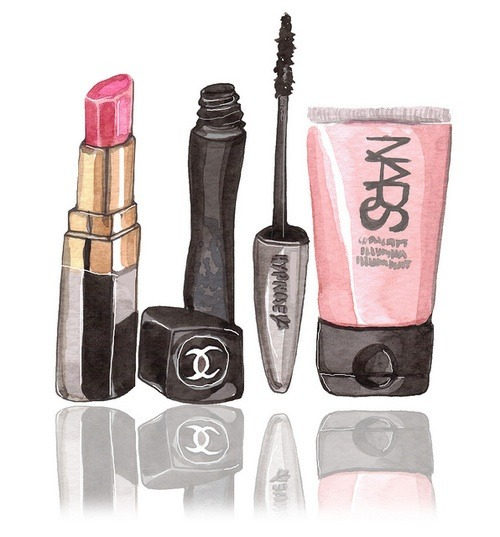
\includegraphics[scale=0.10]{beauty}
 \end{textblock*}
 
 
 \begin{textblock*}{5cm}(7cm,1.2cm)
    
\includegraphics[scale=0.60]{lack}
 \end{textblock*}

\end{frame}
 
